\documentclass[16pts]{report}
\usepackage[utf8]{inputenc}
\usepackage[T1]{fontenc}
\usepackage[francais]{babel}
\usepackage{xcolor}
\usepackage{amsmath}
\usepackage{graphicx}
\usepackage{geometry}
\usepackage{textcomp}

\geometry{hmargin=2.5cm,vmargin=1.5cm}

\begin{document}
\bibliographystyle{unsrt}

\chapter{Contexte}
Il est possible de compiler soi-même un noyau Linux. Cela permet de créer
    un noyau répondant uniquement aux besoins de l’utilisateur. La tâche peut
    être très fastidieuse car les outils permettant de modifier le fichier
    de configuration ne sont pas simples d’utilisation et il est difficile
    de trouver les options que l’on aimerait avoir.

Ce projet à pour but de résoudre ce problème en fournissant un outil permettant
    de simplifier la configuration pour un utilisateur non expert en
    lui permettant d’alléger le noyau à sa guise.

\chapter{Configuration des options du noyau}
La principale tâche à effectuer avant de lancer la compilation du noyau est
    de créer un fichier “.config” comportant toutes les options disponibles
    pour le noyau.  Après avoir récupéré le noyau (sur Kernel.org) on constate
    qu’il n’y a pas de fichier “.config” par défaut. Il faut donc le générer et
    plusieurs options s’offrent à nous :

Récupérer le fichier “.config” d’un noyau sur l’ordinateur que l’on souhaite,
    mais il risque d’y avoir des incompatibilités à cause de la version
    des noyaux.

\begin{description}
    \item[make oldconfig :] Qui permet de récupérer la configuration du noyau
        courant et corrige le problème précédent car en cas d’options
        différentes, le système demandera à l’utilisateur de choisir. Il sera
        difficile d’optimiser ce fichier dans le cas où le noyau courant
        contient des options inutiles.

    \item[make defconfig :] Qui permet de générer un fichier de configuration
        minimale.  C’est la meilleure option permettant d’optimiser son noyau
        sans repartir de zéro.  Malgré tout, il crée une configuration minimale
        générique et non adaptée à la machine de l’utilisateur.
        Le fichier peut donc être optimisé.
\end{description}

Après avoir généré une configuration initiale, il est possible d’utiliser
    différents outils pour la modifier tels que : 

\begin{description}
    \item[make config]      	Un programme en ligne de commande \\
        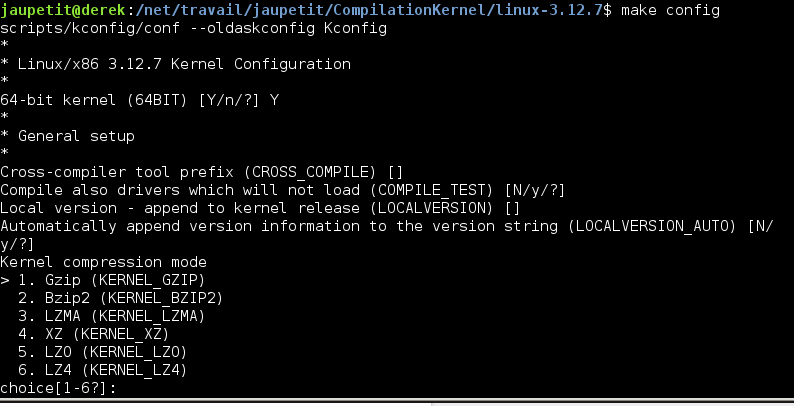
\includegraphics[scale=0.7]{illustrations/configLine.png} \pagebreak
    \item[make menuconfig]      Un programme utilisant ncurse \\ 
        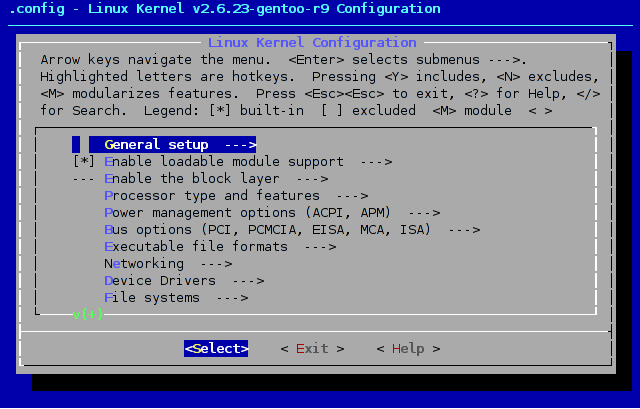
\includegraphics[scale=0.7]{illustrations/menuconfig.png} \\
    \item[make xconfig]     	Un programme utilisant QT \\
        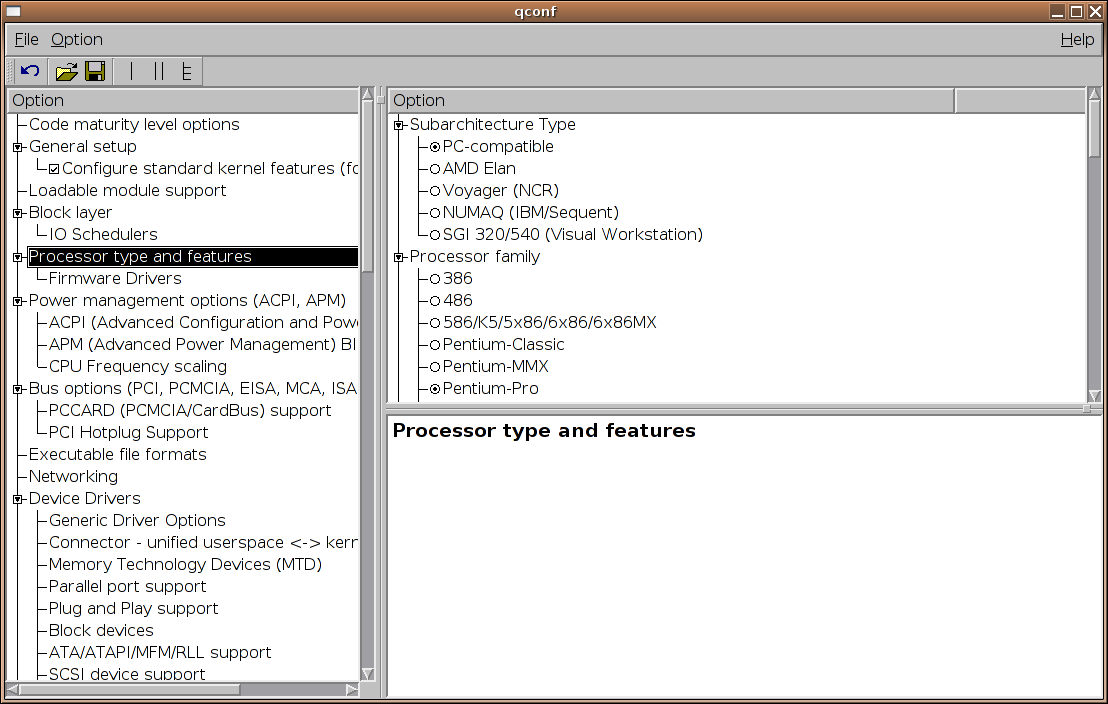
\includegraphics[scale=0.4]{illustrations/xconfig.png} \pagebreak
    \item[make gconfig] 	    Un programme utilisant GTK \\
        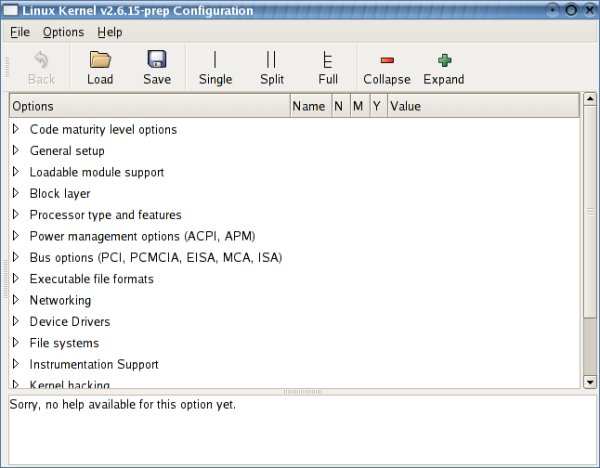
\includegraphics[scale=1]{illustrations/gconfig.jpg} \\
    \item[eCos] , qui permet de configurer les noyaux pour le système
        d’exploitation eCos. C’est une autre source d’information
        sur laquelle se baser. \\ 
        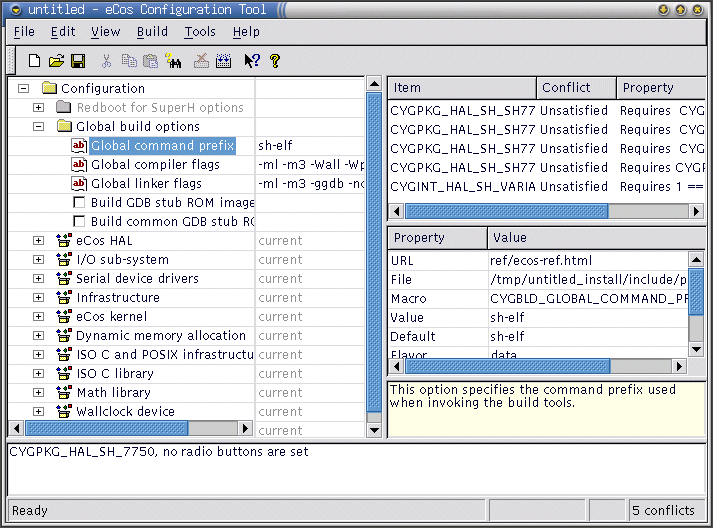
\includegraphics[scale=1.3]{illustrations/eCos_config.png} \pagebreak
	\item[kcheck (kernel check)] permet également de configurer les options d’un noyau
    	à compiler.
Il propose deux modes :

\begin{description}
    \item[Automatique :] kcheck va tenter de déterminer les options du kernel
        en fonction de la machine sur laquelle il est lancé
    \item[Manuel :] kcheck permet à l’utilisateur de modifier comme bon lui
        semble les différentes options du fichier de configuration du kernel.
\end{description}
    
\includegraphics[scale=0.8]{illustrations/KernelCheck.png}\\
\end{description}

Ensuite, une étude a été réalisée par Kacper Bak et Karim Ali de
    l’université Waterloo afin d’améliorer la convivialité de la configuration
    d’un noyau Linux : http://gsd.uwaterloo.ca/node/294

Ceci a permis de mieux cerner les besoins des utilisateurs en observant
    leurs difficultés à utiliser les outils existants. Ils ont réalisé
    un prototype qu’ils ont fait tester et qu’ils ont amélioré afin d’obtenir
    le squelette d’un outil facilitant la configuration d’un noyau Linux. \\

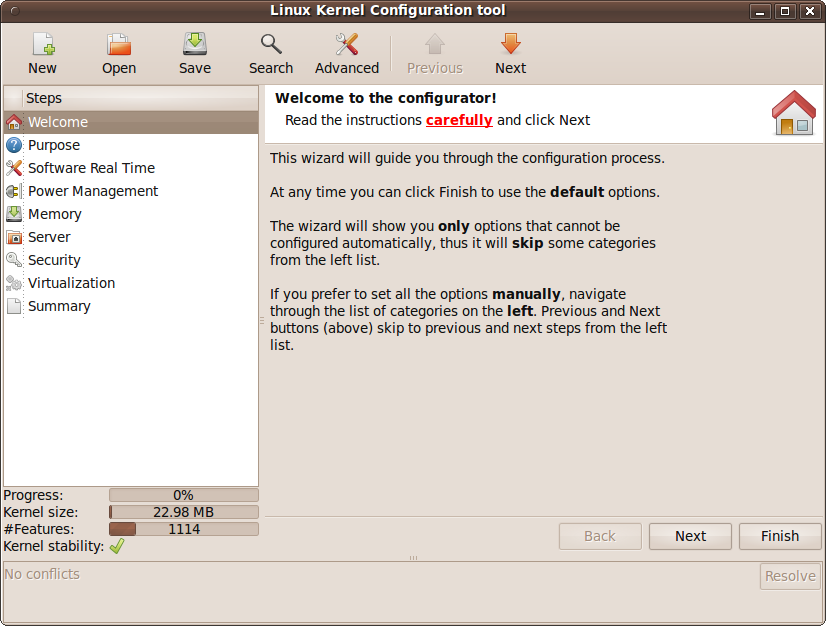
\includegraphics[scale=0.6]{illustrations/lkc-config.png} \\

Leur projet a donc abouti sur un prototype non fonctionnel.
    L’ergonomie de leur application sera une grande source d’inspiration
    pour nous de par les avis qu’ils ont récoltés auprès d’utilisateurs.

\chapter{Difficultés de la configuration :}

Il existe plusieurs raisons qui font que la configuration des options d’un noyau
    est une tâche fastidieuse et difficile :

Tout d’abord, le principal problème se situe au niveau des conflits et
    des dépendances entre les options. En effet, celles-ci peuvent
    être dépendantes d’autres options ou même exclusives, c’est à dire que si
    une option est sélectionnée, une autre peut ne plus l’être.
    Le problème de certains des outils actuels est que les options en conflit
    avec les options actuelles ne sont plus visibles. Donc lorsque l’on cherche
    une option précise qui n’est plus affichée et que l’on ne sait pas quelle
    précédente option est en conflit avec elle, il est très difficile de
    corriger cette erreur.

Enfin, il est compliqué pour un utilisateur non expert de trouver une
    option précise sans la connaître parfaitement. Le nom de cette option
    ne représente pas toujours très bien sa fonction, ce qui fait que
    la recherche des options dans l’outil n’est pas aisée.
    On constate qu’il y a une aide pour chacune des options et
    il est dommage que la recherche par mots-clés ne s’effectue pas également
    sur l’aide des fonctions.

\bibliography{./bibliographie}
\end{document}
